\subsection{Exercise 1}
A company makes two products (X and Y) using two machines (A and B). Each unit of X that is produced requires 50 minutes processing time on machine A and 30 minutes processing time on machine B. Each unit of Y that is produced requires 24 minutes processing time on machine A and 33 minutes processing time on machine B.

At the start of the current week there are 30 units of X and 90 units of Y in stock. Available processing time on machine A is forecast to be 40 hours and on machine B is forecast to be 35 hours.

The demand for X in the current week is forecast to be 75 units and for Y is forecast to be 95 units. Company policy is to maximise the combined sum of the units of X and the units of Y in stock at the end of the week.

\begin{equation}
    \begin{aligned}
        \text{Maximize} \quad   & X + Y                       \\
        \text{Subject to} \quad & 50X + 24Y \leq 40 \times 60 \\
                                & 30X + 33Y \leq 35 \times 60 \\
                                & X + 30 \ge 75               \\
                                & Y + 90 \ge 95               \\
                                & X, Y \geq 0
    \end{aligned}
\end{equation}
Rewrited in slack form and simplified this is equivalent to:
\begin{equation}
    \begin{aligned}
        \text{Minimize} \quad   & -X - Y                          \\
        \text{Subject to} \quad & 50X + 24Y + S_1 = 2400          \\
                                & 30X + 33Y + S_2 = 2100          \\
                                & -X + S_3 = -45                  \\
                                & -Y + S_4 = -5                   \\
                                & X, Y, S_1, S_2, S_3, S_4 \geq 0
    \end{aligned}
\end{equation}
The simplex method was used to solve this problem and the result was $X = 45$, $Y = 6.25$.

\subsection{Exercise 2}
A factory manufactures chairs and tables, each requiring the use of three operations: Cutting, Assembly, and Finishing. The first operation can be used at most 40 hours; the second at most 42 hours; and the third at most 25 hours. A chair requires 1 hour of cutting, 2 hours of assembly, and 1 hour of finishing; a table needs 2 hours of cutting, 1 hour of assembly, and 1 hour of finishing. If the profit is 20 per unit for a chair and 30 for a table, how many units of each should be manufactured to maximize profit?

\begin{equation}
    \begin{aligned}
        \text{Maximize} \quad   & 20X_1 + 30X_2      \\
        \text{Subject to} \quad & X_1 + 2X_2 \leq 40 \\
                                & 2X_1 + X_2 \leq 42 \\
                                & X_1 + X_2 \leq 25  \\
                                & X, Y \geq 0
    \end{aligned}
\end{equation}
Rewrited in slack form and simplified this is equivalent to:
\begin{equation}
    \begin{aligned}
        \text{Minimize} \quad   & -20X_1 - 30X_2                 \\
        \text{Subject to} \quad & X_1 + 2X_2 + S_1 = 40          \\
                                & 2X_1 + X_2 + S_2 = 42          \\
                                & X_1 + X_2 + S_3 = 25           \\
                                & X_1, X_2, S_1, S_2, S_3 \geq 0
    \end{aligned}
\end{equation}

The simplex method was used to solve this problem and the result was $X_1 = 10$, $X_2 = 15$.
\begin{figure}
    \centering
    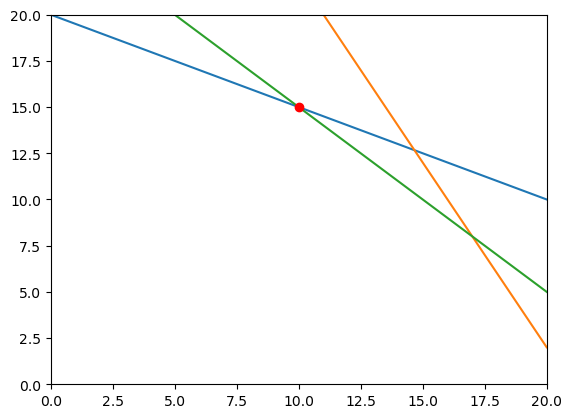
\includegraphics[width=0.8\textwidth]{lab10/imgs/ex2.png}
    \label{fig:lab10-ex2}
\end{figure}

\subsection{Exercise 3}
A mutual fund has \$ 100,000 to be invested over a three year horizon.
Three investment options are available:

\begin{enumerate}
    \item Annuity: the fund can pay a same amount of new capital at the beginning of each of three years and receive a payoff of 130\% of total capital invested at the end of the third year. Once the mutual fund decides to invest in this annuity, it has to keep investing in all subsequent years in the three year horizon.
    \item Bank account: the fund can deposit any amount into a bank at the beginning of each year and receive its capital plus 6\% interest at the end of that year. In addition, the mutual fund is permitted to borrow no more than \$20,000 at the beginning of each year and is asked to pay back the amount borrowed plus 6\% interest at the end of the year. The mutual fund can choose whether to deposit or borrow at the beginning of each year.
    \item Corporate bond: At the beginning of the second year, a corporate bond becomes available. The fund can buy an amount that is no more than \$50,000 of this bond at the beginning of the second year and at the end of the third year receive a payout of 130\% of the amount invested in the bond.
\end{enumerate}
The mutual fund’s objective is to maximize total payout that it owns at the end of the third year.

\begin{equation}
    \begin{aligned}
        \text{Maximize} \quad   & 3.9X_1 + 1.06X_4 + 1.3X_5  & \text{3*1.3 annuity + 1.06 deposit year 3 + 1.3 bond } \\
        \text{Subject to} \quad & - X_1 - X_2 = - 100K      & \text{spend at most 100K in annuity and deposit}        \\
                                & - X_1 + 1.06x_2 - X_3 - X_5 = 0 & \text{spend for annuity, bond and deposit, get capital}        \\
                                & - X_1 + 1.06x_2 - X_4 = 0       & \text{spend for annuity and deposit, get capital}        \\
                                & X_2, X_3, X_4 \ge -20K   & \text{at most 20K deposit in bank}        \\
                                & X_5 \leq 50K             & \text{at most 50K for bond}         \\
                                & X_1, X_5 \geq 0                 &
    \end{aligned}
\end{equation}
where $X_1$ is the total amount to put in the annuity, $X_2, X_3, X_4$ are the bank deposit balances ant the beginning of the three year and $X_5$ is the amount inversted in the corporate bond.

The simplex method was used and the result was
\begin{equation}
    \begin{aligned}
        X_1 = 24930, X_2 = 75070, X_3 = 4649, X_4 = -20000, X_5 = 50000
    \end{aligned}
\end{equation}
